%% LyX 2.0.8.1 created this file.  For more info, see http://www.lyx.org/.
%% Do not edit unless you really know what you are doing.
\documentclass[english]{paper}
\usepackage[T1]{fontenc}
\usepackage[latin9]{inputenc}
\usepackage{color}
\usepackage{array}
\usepackage{textcomp}
\usepackage{multirow}
\usepackage{graphicx}

\makeatletter

%%%%%%%%%%%%%%%%%%%%%%%%%%%%%% LyX specific LaTeX commands.
%% Because html converters don't know tabularnewline
\providecommand{\tabularnewline}{\\}
%% A simple dot to overcome graphicx limitations
\newcommand{\lyxdot}{.}

\floatstyle{}
\newfloat{}{}{}
\providecommand{\name}{}
\floatname{}{\protect\name}

\makeatother

\usepackage{babel}
\begin{document}

\section{Introduction}

Ever since Darwin's theory of evolution was proposed, cooperative
traits in animals and humans were challenging to explain. In order
to do so, Darwin's theory incorporates two novel kinds of extensions:
the genetically kinship theory that Hamilton grounded mathematically
(Hamilton,1964) and the reciprocal altruism theory (Trivers, 1971).
Both appended theories are capable to explain social altruism behavior
through natural selection. In evolutionary biology, reciprocal altruism
is a behavior whereby an organism performs a costly act that benefits
another organism with the expectation that the recipient will act
similarly later time or even in the next generation. 

The kinship theory that after landed on kin Selection and Maynar Smith
use in first time (Smith,64), talk about, on knowledge of the genetic
relationships of the organism involved, how altruistic behavior between
closely related individuals can be selected though natural selection.
This theory does not considers the altruistic act among distantly
related organisms whereas Triver's theroy does. The term \textquotedblleft{}reciprocal
altruism\textquotedblright{} was first used by Trivers to refer to
this type of behavior and therefore explain how selection favors altruistic
behaviors in the long run when there is reciprocity in the population
. Some of the most relevant and reliable examples about this type
of cooperation are the Wilkinson studies in reciprocal food sharing
behavior in vampires bats (Desmodus rotundus), (Wilkinson, 1984).
In these experiments, animals share a part of the harvested food only
to a partner that previously shared with them. Other examples, .... 

Different conditions must be fulfilled to ensure that reciprocally
altruistic behaviors will be selected. Wilkinson makes a clear summary
of these conditions : (1) the behavior must reduce a donor\textquoteright{}s
fitness relative to the selfish alternative, (2) the fitness of the
recipient must be elevated relative to a non-recipient, (3) performance
of the behavior must not depend on receipt of an immediate benefit,
(4) a mechanism for detecting individuals who receive benefits but
never pay altruistic costs has to exist, and (5) a large but indefinite
number of opportunities to exchange aid must exist within each individual\textquoteright{}s
lifetime (Wilkinson, 1987). 

Research on cooperative behaviors between non-related organisms has
gained a new impulse since Trivers connected reciprocal altruism behaviors
with the famous mathematical Prisoner's Dilemma (PD) (originally developped
by Merrill Flood and Melvin Dresher 1950). The PD game is one class
of 2x2 game that involves two players who must choose between two
options, generally called cooperation and defection. The size of the
reward delivered is established according both player's choice. If
both chose the cooperation option both get payed a certain amount
R (reward), and if both chose defection they both get payed a smaller
reward P (punishment) than R. However if one cooperates and the second
player defects, the first one gets payed S (sucker) and other receives
the best amount T (temptation) where the pay-off matrix maintains
the inequality T>R>P>S. 

Both the iterated Prisoner's Dilemma (iPD) and the Evolutionary Stable
Strategies (ESS)(von Neumann and Morgenstern, 1944; Nash, 1949) predict,
or suggest, what behavior (strategy) is likely to occur if a ESS is
adopt by the population, in such a way, no minority using a another
strategy can invade (Smith, 1974). When the 2x2 PD is played only
for one time the best ESS is Defeat strategy. Nevertheless, when the
pay-off matrix employed meets 2R>T+P and the game is played an indefinite
numbers of times, the best strategy is mutual cooperation. e.i. if
one stop reciprocity behavior the best option change to defeat. Axelrod
and Hamilton (1981) showed that some organism's symbiosis can be understood
through the reciprocal altruism's model and if organisms can remember
the outcome of at least one previous interaction and they are able
to recognize different partners, then the strategies situation includes
a much richer set of possibilities. They present a ESS for iPD that
combines robustness and stability with initial viability, called TIT
FOR TAT. This strategy arised as the winner strategy, submitted by
Anatol Rapoport, in the Robert Axelrod's computer tournament, because
it can survive invations from other strategies. The highly simple
strategy consists in cooperating on the first move and then doing
whatever the opponent did on the preceding move. .............. 

Thus, many experimenters have tried to understand different aspects
of reciprocal altruism behavior in animals and whether non-human animals
with less cognitive abilities can solve iPD. Green, Price and Hamburger
(1995) assessed the iPD game on pigeons and observed that birds are
very impulsive and prefer small immediate rewards rather than big,
long-term, delayed rewards. Stevens and Stephens (2003) trained blue
jays (Cyanocitta cristata) using four different pay-off matrices,
where one of them was the iPD matrix, with a special dual operant
box. This study found little cooperation in PD treatment and this
findings suggest that blue jays don't cooperate when immediate benefit
is available (defect only), even if a long-term benefit may exist.
Then Steven and colleages (2002 and 2005) inspired by the low levels
of cooperation observed (Gardner et al., 1984; Clements and Stephens,
1995; Flood et al., 1983; Green et al., 1995) proposed assess over
iPD frame to the effect of a pay-off accumulation and temporal clumping
treatment to iPD game using blue jays in an apparatus that consisted
of side by side V-shaped compartments. They found that combining both
accumulation and clumping treatment birds showed a level of cooperation
that scarcely surpassed chance choice. However, Danchin and colleages
(2006) criticized the Steven's experiment arguing that each accumulation
block the iPD payoff matrix becomes stag hung matrix (whereby the
temptation outcome, T, leave to be the best reward, R>T\ensuremath{\ge}P>S)
because the bird quantify the effective amount after four trials.
Adams and Mesterton-Gibbons pointed out that in a different study
by Stevens And colleages (2002) birds care less about the immediacy
of reward if seeds accumulation in a transparent food tray for some
time before being delivered. 

Moreover, Mendres and Waal(2000) and Waal(2000), used a pulling task
in capuchin monkeys (Cebus apella) and a chamber divided with mesh
to test cooperation. As a result, monkeys could adjust pulling task
behavior according to their partner's presence and in turn the food
shared behavior depended of quality of own and partner foods. Similarly,
using a pulling task to give food to a partner and receive from a
altruistic partner Hause and colleagues(2003) evaluated altruistic
food giving behavior where sharing food through the mesh was not allowed
over genetically unrelated cotton-top tamarin mokeys(Saguinus oedipus)
and showed that monkeys give more or less foods to their partners
taking into account whom was altruistic and whom not. 

Knowing that primates have high psychological capabilities (cita)
we can expect that these animals can learn reciprocal altruism despite
of not performing this behavior in the wild. It's interesting then
to investigatee whether animals with less cognitive habilities can
learn reciprocal altruism. Using silimar protocols than the ones used
for primates, Rutte and Taborsky (2007) assessed generalized reciprocity
in female rats (Rattus norvegicus) by means of a alternating pulling
task in a Wall and Menders chamber adapted for rats. In this protocol,
the focal rats adopt a role of either \textquotedblleft{}helper\textquotedblright{}
in which they give food to a partner or \textquotedblleft{}receiver\textquotedblright{}
where thay take food from a partner. Generalized reciprocity is kind
of reciprocal altruism between unrelated individuals where individual
make altruistic behaviors by previous social experience irrespective
of partner identity. The Taborsky's experiment was carried out with
two phases: in the first, pre-training, phase the experimenter taught
focal rats to perform alternating reciprocal task and in the second
phase that after receive help or not for several days from differents
partners were paired with a new partner in role of potential helper.
They observe that the rats pull more frequently when they previously
received interaction with a food-givers partner. From an operant conditioning
perspective, we believe they have actually assessed extinction rate
of pulling behavior after focal rats have or not received food for
several days rather than rising the frequency of behavior by interaction
between players. Then, Rutte and Taborsky (2008) evaluate direct versus
generalized reciprocity using the same experimental set up. Direct
reciprocity is a kind of reciprocate interaction in which a subject
A cooperates with B on account of B previously cooperated with A.
They observe that the pull rate is higher and its delay to pull is
lower on direct reciprocity than generalized. This means that a know
opponent is a more powerfull stimulus than unknown. Taborsky and colleagues(2012)
have shown that rats reduced the pulling rate with increasing resistance
to pull and Dolivo and Taborsky (2015) evidennce that rats take into
account the quality of the food received from the opponent in future
cooperation (pulling). 

-creo que este p�rrafo no va----In our search for altruistic behavior
in non-humans and non-primate animals we maybe demur that rats behavior
in Taborsky's experiment didn't meet all of the conditions for reciprocal
altruistic behavior. Because rats don't receive punishment for either
punishment or temptation outcomes they rather assessed a different
type of reciprocity----- 

Reciprocal altruism has been widely tested by iPD, where the individual's
decision rules can be described by a transition vector t, r, p, s
that reflects the probability of cooperation when the previous trials
resulted in outcomes of R, T, S or P, respectively (Stevens and Stephens,2004).
If every component of this vector is 0.5, the agent's decision rule
is random irrespective of the last outcome. Part of the experiments
sets developed by Wood and colleagues (2016) were aimed to measure
reciprocal altruism in Long Evans male and female rats using iPD.
They used an operant chamber divided in halves by a removable mesh
and equipped with retractable levers and stimulus light. As a result,
they show a 60\% of altruistic behavior on male rats, barely surpassing
chance choice. 

To test whether rats have the ability to solve the iPD game when faced
to altruist opponent, is necessary to force TIT FOR TAT behavior on
the opponent (Stevens and Stephens, 2002; St-Pierre et al., 2009;
Viana et al., 2010). In Moita's study (Viana et al., 2010) mimicking
a tit-for-tat strategy on the opponent in a double T-maze chamber
was not enough to reach high levels of cooperation. We further analyzed
their Markov chain diagram and observed that the strategy performed
by rats was more selfish than cooperative because it adopted an alternating
decision's rule among sucker and temptation outcomes. 

The rats often develop on social groups and studies have demonstrated
that they prefer social reward rather than being rewarded in isolation.
The result showed that he rats had a tendency to perform pro-social
acts barely over the chance (Moita, 2015;Kalenscher, 2015). 

Why all iPD-based studies haven't found high levels of reciprocity?
In the aforementioned previous studies, rats don't learn iPD probably
due to the fact that the test box and stimulus contingency are inadequate
for its natural expectation, i.e. the rat maybe has the ability to
achieve a approximated optimal solution but for example the length
of time used to make the contingency is longer than what rats can
keep in mind or maybe they don't realized the real difference within
outcomes in the pay-off matrix. 

Given these consideration, the present study was conduct to assess
reciprocal altruism behaviors using a particular structure that combine
iPD matrix pay-off and delay's punishment and a tit for tat opponent's
strategy. We found that this combination achieve high level of reciprocal
altruism behavior in rats.


\section{Material and Method}

All experimental procedures were approved by the ethics committee
of the IByME-CONICET and were conducted according to the NIH Guide
for Care and Use of Laboratory Animals.2.1 Subjects and Housing


\subsection{Subjects and Housing}


\subsubsection{Subject}

Two groups of male LongEvans rats (300\textendash{}330 g) of two months
of age were provided by the IBYME-CONICET. Twelves males were subjects
and six (Nstooge=6) identical rats were opponents. At weaning time
all subjects were housed in groups of two rats per cage to allow social
interaction, whereas each stooge was housed in single individual cages.
We had 12 stainless-steel cages altogether with sawdust as bedding
and metal lids. All rats were food restricted to maintain animals
at between 90-95\% or 80-85\% of free feeding body weight for subjects
and stooges respectively. All animals were kept in a well-ventilated,
temperature-controlled room (22 \textpm{} 2 \textdegree{}C) with a
12/12 h light/dark cycle (lights on at 8 am). Tap water was available
ad libitum. To ensure that animals obtained sufficient food to survive,
we provided supplementary food (at 22hs) for any rats that obtained
the average amount of pellet to maintain body weight. 

The subject was named in succesive order: 1A, 2A, 3A, 4A, 5A, 6A,
7A, 8A, 9A, 10A, 3B, 4B.


\subsubsection{Housing}

All behavioral procedures were performed during the light phase of
the light/dark cycle, using a standard operant chambers (MED associates
Inc., USA) with Med PC IV software suit (Product SOF-735) and PCI
Operating Package for up to Eight Chambers (Product MED-SYST-8) equipped
with control of multiple devices SmartCtrl (Product DIG-716B) and
pedestal mount pellet dispenser for rat, 45mg (Product ENV-203-45)
and standard operant chambers (Product ENV 008). White noise with
a flat power spectral density was used to reduce sensibility to ambient
noise. The training was perform on a single standard operant chamber
equipped with tree retractable levers and tree stimulus light over
each lever, and in the back wall placed a illuminated feeder. The
experiment was conducted in special ad hoc dual chamber. We placed
two Med association standard operant chambers facing each other in
such manner that each rat could make olfactory and eye contact through
metal windows (FIGURA 1 CAJAS). Each standard chamber was equipped
with: two not retractable levers at the sides of the same wall and
two stimulus light were placed over each levers, and in the center
put a illuminated feeder. The boxes were faced by the wall that has
levers and stimulus light. To allow the contact among rats we placed
a aluminum rectangular windows below each levers. The window's height
were such that the lever's height was 80\% of maximum height of the
forepaws while rearing (F. Cabrera et al., 2013). The subject's feeder
placed in same wall and the opponent's feeder placed in back wall.
Each feeders were equipped with a stimulus light that turn on when
foods is coming. 


\subsection{Procedures}

During the whole duration of experiment, every actor were trained
for 2 session per day for all handing, habituation, training and iPD
experiment sessions. The 5 second inter-trial interval(ITI) was used
and each trial duration was 45 second. The standard experiment session
had 30 trials. 


\subsubsection{Training procedure}


\paragraph{Handing}

At weaning time when the animals were moved to housing room started
a handing procedure to decrease the stress by experimenter manipulation
and finished when animals had 60 days old. 


\paragraph{Habituation}

The animals were habituated to the single and double operant chamber
for a days in session of 3 minute. In this treatment, there were either
no stimulus-reward contingencies or reward, only a back-light that
marked the beginning and the end of sessions.


\paragraph{Magazine}

To learn the place in which the food is given, the rat were exposed
for a days to a ``\emph{Magazine}'' procedure in the single chamber.
It consisted in variable ratio reinforcement scheduler. 


\paragraph{Shaping}

The pressing lever training on rats was done through a successive
approximations procedure, ``\emph{Shaping}'' (Mazur, 1994, page
122) on a single chamber. The chamber was equipped as described above
and was added a external lever. In this training, the external lever
was manipulated by the operator to give reward as the rat go to the
goal and finally when press lever. When the rat learned to press the
lever after light onset, the operator left to gave reward with his
lever. It training finished when the rat made the task for at least
two session. Trials procedure: each trial began when the center stimulus
light was turned on and the lever below it was ejected, then if either
inner or outer levers wasn't pressed and 45 second had elapsed, the
trials finished and not reward was given. But nevertheless, if either
inner or outer levers was pressed, the light turn-off and the feeder's
light was turned on, one second later a 45mg pellet is automatically
dispensed, when 5 second elapsed all light were turn off and the lever
was retracted, finally 5 second ITI started. The procedure was performed
during 3 days or until the rats met task goal.

Following, we exposed the rat to the same task but now the center
lever during the session never more was retracted, the lever ejected
at first trials and retracted at the last trials. In this training,
when the rat pressed lever on ITI was punished with 2 second delays
added to 5 second of ITI. This procedure went on for tree days or
until pressing rate was below one per trials.


\paragraph{Basic toggle task for subject}

The subject rats group was exposed to a training called ``toggle
8x8'' in dual iPD chamber. The purposed of the training was show
that two lever exist and balance rat lever's preference. The experiment
was performed by 2 days in which on first day a rat use chamber 1
and on day 2 used chamber 2. This last allow not placed preference.
The chamber communication windows were closed and any contact was
suppressed. Each rat had two lever option and two light stimulus.
When session started since the first to eighth trials only one pair
stimulus light and lever worked and the next 8 trials(9-16) the another
pair light-lever worked. What pair light lever started was randomly
and in the second day was maintained in the same way. The trials procedure
was identical to the previous one in the shaping.


\paragraph{Mimic tit for tat for opponent}

The opponent learned to develop a mimic tit for tat strategy by to
learn a basic operant task. The opponent rat group was exposed to
a fixed ratio (FR) schedule in dual operant chamber equipped in the
same way. The pair light-lever was randomly assigned in each trials
along the session. In this training, the rat must to press the lever
that had light turned on. The other lever did not work during the
trials and on the next trials the light-lever pair that worked was
pseudo-randomly assigned. Pseudo-randomly means that the assigned
was random but not allowed the same assigned for more than four time.
The training was developed during five days and the FR schedule was
increased step by step: day 1� the FR=2 and day 2� to 3� the FR=3,
then day 4� the FR=4 and finally day 5� the FR=5. If the rat press
the lever on ITI time received 2'' second delay added ITI time as
punishment. 


\subsubsection{Iterated Prisoner's Dilemma Procedure}

The main experiment was designed to study the reciprocal cooperation
lever in a iterated prisioner's dilemma game. We used a pay-off matrix
in which T>R>P>S. The T and R outcomes were positive reinforcement
and P and S was punishment. The matrix coefficient are shown in TABLE
1. Thus, If opponent choose the cooperation option (C) and the subject
choose C or defection option (D), the subject received one pellet
or 2 pellet, respectability. When the Opponent choose D and the subject
choose C or D, the subject received 8'' or 4'' delay of punishment
and no pellet in this trial. The opponent strategy was conducted by
place in which the stimulus was lighting, e.i. the opponent didn't
choose freely and the side where light was turn on, the opponent pressed
the lever. The amount pellet preference was test previously and the
rat shown more preferences for 2 pellet than 1 pellet. The delay discrimination
had been tested in \textcolor{red}{PAPER DE SELF CONTROL EN RATAS. }

\begin{table}
\caption{Prisioner's Dilemma Pay-off Matrix}


\begin{tabular}{|c|cc|}
\hline 
\multirow{2}{*}{} & \multicolumn{2}{c|}{Opponent choice}\tabularnewline
\cline{2-3} 
 & C & D\tabularnewline
\hline 
Subject choice & \multicolumn{2}{c|}{}\tabularnewline
\cline{1-1} 
\multicolumn{1}{|c||}{C} & 1 pellet & 8'' delay\tabularnewline
\multicolumn{1}{|c||}{D} & 2 pellets & 4'' delay\tabularnewline
\hline 
\end{tabular}
\end{table}


In iPD experiment used a dual chamber without neither center lever
and center light. The windows cover was removed. The rats had only
two lever option and the contact between chamber was restored. There
was one chamber for the subject and one for the opponent fixed during
all the experiment, see the figure xxx(figura 1 de ARRIBA). 

The main experiment was conducted for 10 days and 2 session per day.
The session consisted in 30 trials. For individual subject, the experiment
was stopped, if the average behavior didn't change along ten consecutive
sessions. To some subject was exposed more than 20 days when rise
its behavior tendency. 


\subsubsection{Typical Trial Structure}

The sequence of events within a single trial was as follows. (1) The
stimulus light was turned on stating that trails was started. The
focal rats had both lights turned on (this was done throughout the
iPD experiment) and the opponent only one for the tit for tat strategy.
(2)after both rats done their response, the light was turned off and
the rewards computed. (3) The feeder's light was lighting one second
before a reward was delivered. If the opponent pressed the lever always
received one pellet irrespective the focal rat's choice. If punishment
was assigned, the focal rat feeder's light remained off and the punishment
time started, but the opponent's feed was lighted and its one pellet
reward was delivered. (5) After either five second eating time expired
or punishment time complete, all light was turned off. Then, the focal
and opponent waited for fixed ITI time. The next trials started.


\subsection{Statistical Analysis}

Al statistical analysis were performed using statistic library from
octave open source software. 


\subsubsection{Stability of cooperation}

To analysis the choice stability of rats in the iterated game, we
used the last 10 session as a pool of data due to the rat's behaviors
had reached a plateau.


\subsubsection{Probability of cooperation after outcomes}

The animals probability to cooperate after each outcomes was assess
using a chi square test. The probability of cooperation given specific
outcomes in last trial was compared from chance, 0.5. We performed
a Chi-square goodness of fit test with bonferroni corrected value
of 0.05/n.


\subsubsection{Rate of difference outcomes}

we used friedman test and postmultiple post-hoc pairwise comparisons
using the Nemenyi\textquoteright{}s procedure/Two-tailed tests were
performed, with the Bonferroni corrected a value of 0.0083.


\subsubsection{Markov chain diagram}

We compute the strategies for each rats by diagram of probability
of transition between outcome. The outcomes were T (temptation) in
which 


\section{Results}

The experiment result are show below. To assessing whether a subject
was abled to solve the iPD game, we first need to know whether either
the subject adopt some strategy or play in random mode. We compute
the rat behavior from data of last ten session at the end of the experiment.
A strategy was defined by a transition vector that reflects the probability
of cooperation when the previous trials resulted in outcomes of R,
T, S or P, respectively ($v=[p(c|t),p(c|r),p(c|p),p(c|s)]$). The
end of experiment for each rat was extended beyond 20 session in order
to the rat was progressively finding some strategy. The rat that maintained
a random strategy beyond 20 session was deserted. When the rat maintained
a not random behavior at least for ten session, the experiment was
stop. To test if rat strategy differs from chance strategy (v={[}.5
.5 .5 .5{]}), we perform a $\chi{}^{2}$ goodness of fit test on last
ten session.

After compute the parameter $\chi{}^{2}$with bonferroni correction
for each rat we obtained two group of subject. Those who adopted some
strategy and those who did not. The figure (X) shows the mean of cooperation
for all rats and the asterisks marks denoted subject that had significant
difference respect the chance. The subject 2A, 4A, 5A, 6A were removed
from data pool because they not had a fixed strategy (See Supplementary
materials for the graph of markov chain with probabilities of transition).
Since the table \ref{table_meanAndstrategies} we can see that there
is a group of 8 rats with had a fixed no random strategy.



\begin{label}
\label{fig_meansAndSignificance}\caption{\textbf{\scriptsize{}Mean and }{\scriptsize{}$\chi{}^{2}$}\textbf{\scriptsize{}test}{\scriptsize{}:
The rats with 95\% of free feeding body weight played under a matrix
pay-off T=2, R=1,P=4''delay, S=8''delay against a TFT opponent.
We show means of the numbers of times rats chose the cooperate option.
The Asterix denote when strategy adopted by a rat had significant
difference from chance strategy. }}


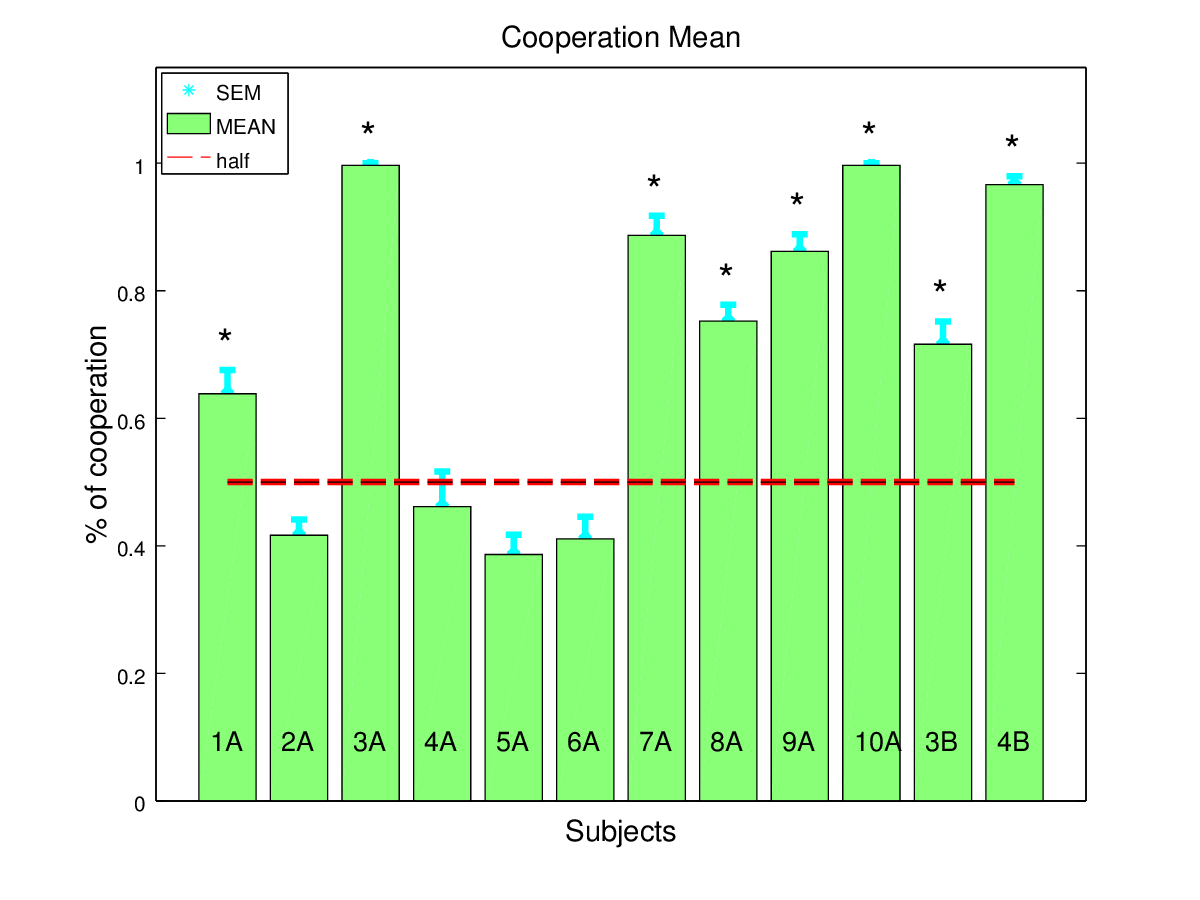
\includegraphics[draft,width=1\paperwidth]{/home/guille/Documents/experimento/Experimento---iPD/ExtraerDatos/figura_iPD_1_2_9s_13s/fig_finales/cooperation_mean_with_significant}
\end{label}


\begin{table}
\label{table_meanAndstrategies}\caption{We show the mean of cooperation and the values of probabilities of
cooperation given each outcomes. The $\chi^{2}test$ with bonferroni
correction results and significance show the subject that devoloped
a specific strategy. The subject underlined and in blue text color
had significant different respect random strategy. }


{\scriptsize{}}%
\begin{tabular}{|c|c|c|c|c|c|c|c|}
\hline 
 & {\scriptsize{}Mean} & \multicolumn{4}{c|}{Strategies} &  & \tabularnewline
\cline{1-1} \cline{3-8} 
{\scriptsize{}Subject} & {\scriptsize{}cooperation} & {\tiny{}$p(c|T)$} & {\tiny{}$p(c|R)$} & {\tiny{}$p(c|P)$} & {\tiny{}$p(c|S)$} & {\tiny{}$\chi_{bonferroni}^{2}$} & {\tiny{}$p<0.125$}\tabularnewline
\hline 
\hline 
\textbf{\textcolor{blue}{\emph{\tiny{}1A}}} & \emph{\tiny{}$0.639$} & \emph{\tiny{}$0.525$} & \emph{\tiny{}$0.691$} & \emph{\tiny{}$0.644$} & \emph{\tiny{}$0.667$} & \emph{\tiny{}$17.15$} & \textcolor{blue}{\emph{\tiny{}$6.583e^{-4}$}}\tabularnewline
\hline 
\textbf{\tiny{}2A} & {\tiny{}$0.417$} & {\tiny{}$0.469$} & {\tiny{}$0.408$} & {\tiny{}$0.446$} & {\tiny{}$0.333$} & {\tiny{}$8.02$} & {\tiny{}$0.0456$}\tabularnewline
\hline 
\textbf{\textcolor{blue}{\tiny{}3A}} & {\tiny{}$0.997$} & {\tiny{}$1$} & {\tiny{}$0.996$} & {\tiny{}$0$} & {\tiny{}$1$} & {\tiny{}$199.30$} & \textcolor{blue}{\tiny{}$0.0000$}\tabularnewline
\hline 
\textbf{\tiny{}4A} & {\tiny{}$0.461$} & {\tiny{}$0.5$} & {\tiny{}$0.625$} & {\tiny{}$0.348$} & {\tiny{}$0.403$} & {\tiny{}$9.60$} & {\tiny{}$0.0223$}\tabularnewline
\hline 
\textbf{\tiny{}5A} & {\tiny{}$0.386$} & {\tiny{}$0.359$} & {\tiny{}$0.408$} & {\tiny{}$0.351$} & {\tiny{}$0.459$} & {\tiny{}$10.42$} & {\tiny{}$0.0152$}\tabularnewline
\hline 
\textbf{\tiny{}6A} & {\tiny{}$0.411$} & {\tiny{}$0.493$} & {\tiny{}$0.37$} & {\tiny{}$0.381$} & {\tiny{}$0.394$} & {\tiny{}$8.45$} & {\tiny{}$0.0375$}\tabularnewline
\hline 
\textbf{\textcolor{blue}{\tiny{}7A}} & {\tiny{}$0.886$} & {\tiny{}$0.778$} & {\tiny{}$0.904$} & {\tiny{}$0.857$} & {\tiny{}$0.885$} & {\tiny{}$103.23$} & \textcolor{blue}{\tiny{}$0.0000$}\tabularnewline
\hline 
\textbf{\textcolor{blue}{\tiny{}8A}} & {\tiny{}$0.762$} & {\tiny{}$0.638$} & {\tiny{}$0.75$} & {\tiny{}$0.682$} & {\tiny{}$0.864$} & {\tiny{}$49.38$} & \textcolor{blue}{\tiny{}$1.081e^{-10}$}\tabularnewline
\hline 
\textbf{\textcolor{blue}{\tiny{}9A}} & {\tiny{}$0.862$} & {\tiny{}$0.781$} & {\tiny{}$0.851$} & {\tiny{}$0.778$} & {\tiny{}$1$} & {\tiny{}$105.91$} & \textcolor{blue}{\tiny{}$0.0000$}\tabularnewline
\hline 
\textbf{\textcolor{blue}{\tiny{}10A}} & {\tiny{}$0.997$} & {\tiny{}$1$} & {\tiny{}$0.996$} & {\tiny{}$0$} & {\tiny{}$1$} & {\tiny{}$199.30$} & \textcolor{blue}{\tiny{}$0.0000$}\tabularnewline
\hline 
\textbf{\textcolor{blue}{\tiny{}3B}} & {\tiny{}$0.715$} & {\tiny{}$0.742$} & {\tiny{}$0.687$} & {\tiny{}$0.842$} & {\tiny{}$0.705$} & {\tiny{}$50.51$} & \textcolor{blue}{\tiny{}$6.217e^{-11}$}\tabularnewline
\hline 
\textbf{\textcolor{blue}{\tiny{}4B}} & {\tiny{}$0.966$} & {\tiny{}$0.889$} & {\tiny{}$0.97$} & {\tiny{}$1$} & {\tiny{}$1$} & {\tiny{}$174.45$} & \textcolor{blue}{\tiny{}$0.0000$}\tabularnewline
\hline 
\end{tabular}
\end{table}


In figure \ref{fig_meansAndSignificance} we show the mean of reward
per subject. The rats with not random strategies got many more reward
than the removed group. But nevertheless, we show that the iPD game
gives to the random strategy group a amount that between 60\% to 70\%
of total reward.

A group of 8 rats that showed a not random strategy and a second group
of 4 rats with a random strategy. The group with random strategy was
disregarded, because these subjects had no information on some behavior.
These group are shown in figura X(media, cadena de markov aplicandole
bondad de ajusta a model al azar). The rats that no exceed the level
of fifty percent of cooperation's choice, showed a random strategy. 

Luegose analizaron la estategias del grupo de 8

,

,

,The figure XX show the graph of markov chain with probabilities of
transition both groups


\section{Discussion}

.receive the double amount of pellet es mas tentados que la mitad.
esp hace que las ratas tiendan a alternar palanca

.

Podemos decir que quiz�s las ratas en esrado salvaje no cooperan por
en una poblaci�n 


\section{Reference}


\section{Supplementary Material}


\end{document}
